Consider the following proportional control system
\begin{center}
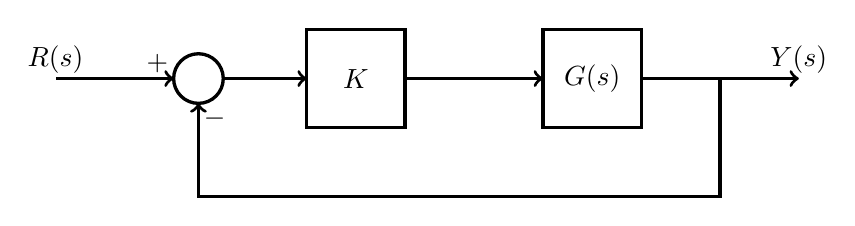
\begin{tikzpicture}[scale=1,inner sep=0pt,outer sep=0pt,very thick,
sysblock/.style={draw,rectangle,inner sep=4pt,minimum width=1.25cm,minimum height=1.25cm,very thick}]

\draw (-2,0) node[draw,circle] (sum1) {$\rule{0pt}{18pt}$};
\draw (0,0) node[sysblock] (K)  {$K$};
\draw (3,0) node[sysblock] (G) {$G(s)$};
\draw[<-] (sum1.180) node[above left=2pt] {$+$} -- ++(-1.5,0) node[above=2pt] {$R(s)$};
\draw[->] (sum1.0) -- (K.180);
\draw[->] (K.0) -- (G.180);
\draw[->] (G.0) --  ++(2,0) node[above=2pt] {$Y(s)$};
\draw[->] (G.0) -- ++(1,0) -- ++(0,-1.5) -| (sum1.-90) node[below right=2pt] {$-$};
\end{tikzpicture}
\end{center}
For a rational transfer function, the {\em relative degree} is the order of the denominator minus the order of the numerator. So for example, $G(s)=\frac{1}{s^{3}+2s+2}$ is relative degree 3, while $G(s)=\frac{s^{2}+2s+2}{s^{3}+2s+2}$ is relative degree one. What feature of the root locus can be used to prove the following statement: For any system relative degree 3 or higher, there exists a $K_{0}$ such that the closed loop system is unstable for all $K>K_{0}$?
